% GravExplain
\documentclass[prb,preprint]{revtex4-1} 
% \documentclass[prb,preprint,letterpaper,noeprint,longbibliography,nodoi,footinbib]{revtex4-1} 

% Note that AJP uses the same style as Phys. Rev. B (prb).
% The AIP Style Manual\cite{AIPstylemanual} is an indispensable reference on good physics writing, covering everything from planning and organization to standard spellings and abbreviations.
% Most important of all, please familiarize yourself with the AJP Statement of Editorial Policy,\cite{editorsite} which describes the types of manuscripts that AJP publishes and the audience for which AJP authors are expected to write.
% We look forward to receiving your submission to AJP.
\usepackage[utf8]{inputenc}
\usepackage{amsmath,amssymb,amsthm}
\usepackage{amsfonts}
\usepackage{graphicx}
\usepackage{float}
\usepackage{mathtools}
\usepackage[usenames,dvipsnames]{xcolor}
\usepackage{hyperref}
% \usepackage{siunitx}

\bibliographystyle{apsrev4-2}
% \setlength{\parindent}{0pt}

\newcommand{\jam}{\textcolor{magenta}}
\newcommand{\han}{\textcolor{orange}}


\begin{document}

\title{GravExplain: Continuous gravitational wave data analysis in a table-top experiment}

\author{James W. Gardner}
\email{u6069809@anu.edu.au}
\affiliation{Research School of Physics, Australian National University, 60 Mills Rd, Acton ACT 2601 Australia}

\author{Hannah Middleton}
\email{hannah.middleton@unimelb.edu.au}
\author{Andrew Melatos}
\email{amelatos@unimelb.edu.au}
\affiliation{School of Physics, University of Melbourne, Parkville, VIC, 3010, Australia}
\affiliation{OzGrav-Melbourne, Australian Research Council Centre of Excellence for Gravitational Wave Discovery}

% Summer 2019/2020
\date{\today}

% AJP requires an abstract for all regular article submissions.
\begin{abstract}
Continuous gravitational wave searches use sophisticated statistical techniques to search for signals in noisy data. We demonstrate some of these techniques in a table-top Michelson interferometer. We also create an optical microphone capable of playing back simple recordings of injected audio.
 
\end{abstract}

\maketitle

% cover page that attributes all contributions

\section{Introduction}

% general gw intro
In 2015 gravitational waves were observed for the first time from the merger of two black holes in a binary system.~\cite{GW150914} 
The observation, made by the Laser Interferometer Gravitational-wave Observatory~\citep[LIGO]{AdvancedLIGO:2015}, marked a breakthrough in modern astrophysics and provides a new means to observe the universe. 
Since 2015, the LIGO and Virgo~\cite{AdvancedVirgo:2015} observatories have made numerous detections of binary black hole~\cite{GW151226,GW170104,GW170814} and binary neutron star~\cite{GW170817,GW170817multi,GW190425} mergers. 
In recent years there has been an increased public interest in gravitational-wave science. 
Many gravitational wave research groups around the world have produced demonstrations and activities to aid in explaining this topic to a general audience
Activities range from online data analysis tutorials,~\cite{GWOSC:online,LOSC:2015} hands-on demonstrations, phone apps,~\cite{LaserLabs:online,SciVR:online} and online games,~\cite{BlackHoleHunter:online} to exhibitions,\cite{L2URSSE} artistic interpretation, and musical performance \han{add refs}. 



% what are gws and how do we detect them...
Gravitational waves are a prediction of Einstein's theory of general relativity. 
They are disturbances in spacetime caused by the acceleration of massive objects. 
The effect of gravitational waves is to change distances; a ``stretch and squeeze'' effect. 
Observatories such as LIGO, Virgo, and KAGRA~\cite{KAGRA:2013} are laser interferometers; they use the interference of laser light to measure changes in distance. 
The observatories themselves are extremely complex devices, however they are based on the Michelson interferometer. 
Table-top Michelson interferometers are commonly used by gravitational-wave research groups to demonstrate this science to non-specialist audiences~\cite{ThorLabsIFO,NikhefIFO}\han{add exhibit info when available} and they are often used in undergraduate lab experiments~\cite{UgoliniEtAl:2019}. 


% continuous gws
To date the network of gravitational-wave observatories have observed short-duration transient signals~\cite{GWTC-1:2018,GWOSC:online}. 
However, these observatories are also searching for continuous gravitational waves; persistent, periodic signals which should be present in the data for many months or years. 
A prime target for these searches are rotating neutron stars. 
So far many searches have been made of LIGO and Virgo data, however no detection has been made so far.


% overview
In this article we describe how a Michelson interferometer can be used to demonstrate the search for continuous waves to a general audience. 
The techniques used are very similar to those used by researchers to search for continuous waves in LIGO and Virgo data. 
In section X we describe...... \han{add this in at the end}


% \section{Method and results}
\section{Table-top gravitational wave data science}

\subsection{Michelson interferometry}
% hardware: path difference, virtual thin film interference

\subsection{The webcam method}
% how to analyse video, python OpenCV2

% acknowledge problems: fringe counting, transfer function, coupling


% \section{Results and analysis}
% combined/interwoven results, analysis, and discussion

\subsection{Tracking tones with the Viterbi algorithm}
% explaination and successful application
% \jam{should we introduce viterbi in the introduction, probably?}

% we can do this with both webcam and photodiode

\section{Optical microphone}
% aim of optical microphone: play back injected sounds

The natural succession to tracking simple tones is to try complex audio signals, such as simple chords, and ultimately, music and speech. The Viterbi algorithm is not applicable to these signals, as it is designed to track a single tone signal that slowly, continuously changes frequency. Whereas music and speech consist of many tones that jump frequencies. As such, the interest now is in being able to record and play-back these complex audio signals. Using the interferometer set-up to do makes it an optical microphone, using light to capture sound.

\subsection{The photodiode method}
% advanced method: explain how we capture data

For an optical microphone to be sensitive to speech and music it needs a frequency response far higher than the 30Hz of a standard webcam. Both speech and music need at least kHz response, with speech intelligibility requiring up to 3kHz and music preferably at least 8kHz. This can be addressed by a high-speed webcam, or more simply, by a photodiode.


A photodiode is an electrical component that acts as a regular diode when no light is incident on it (blocking any current flow in the reverse direction), but becomes more and more conductive in the reverse direction as the intensity of incident light increases. Fundamentally, a current is created in the photodiode by the photo-electric effect. Placing a photodiode in reverse-bias over an op-amp creates a photo-detector that will produce a voltage dependent linearly (as a sound approximation) to the incident intensity.


To the interferometer set-up, placing a photodiode anywhere in the interference pattern will record the signal. The signal is independent of the position, up to an initial phase difference, since the interference principle means that all peaks become troughs together (and visa versa). This experiment placed it just off-centre.


The analog signal from the photodiode is captured by an analog-to-digital converter (ADC) connected to the special purpose input (SPI) pins of a Raspberry Pi, in the standard configuration. This digitally samples the signal at roughly 16kHz which introduces the first step of signal processing. Any existing frequency component of the analog signal above the Nyquist frequency of 8kHz would be aliased down into the detected range. To prevent this, an anti-aliasing Sallen-Key filter tuned to 16kHz is included before the ADC. This component attenuates any frequencies above 16kHz, before they get digitally sampled.


All together, the photodiode measuring circuit diagram is shown in Figure~\ref{fig:circuit_diagram} in the appendices. It’s worth noting that it’s not immediately clear what is limiting the sample rate to 16kHz, but it is likely non-optimal reading by the Pi.
% The ADC used (MCP3008) is quoted at 200kHz (or ksps, kilo samples per second).
It is also worth noting that this method does not solve the problems of fringe counting nor speaker coupling.


\subsection{Signals processing: basics}
% transfer function, power-spectral-density

\subsection{Signals processing: filters}
% breakdown of model and all of the filters

% link back, gravitational wave searches also do lots of signal processing

\subsection{Reconstructing music and voice}
% results of processing, likely mixed with above subsection


\section{Conclusions}
% we are able to successfully ...


\appendix

\newpage
\section{Intensity relation derivation}
\begin{align}
    y_0(t) &= A \sin{(k L - \omega t)} \\
    y_1(t) &= A \sin{(k (L + 2 d \cos{\theta}) - \omega t)} \\
    Y(t) &= A \sin{(k L - \omega t)} + A \sin{(k (L + 2 d \cos{\theta}) - \omega t)} \\
    \phi &= 2 k d \cos{\theta} \\
    Y(t) &= A\; \Im\{e^{i (k L - \omega t)} + e^{i (k L + \phi - \omega t)}\} \\
    Y(t) &= A\; \Im\{e^{i (k L + \phi/2 - \phi/2 - \omega t)} + e^{i (k L + \phi/2 + \phi/2 - \omega t)}\} \\    
    Y(t) &= A\; \Im\{e^{i (k L + \phi/2 - \omega t)} (e^{- i \phi/2} + e^{i \phi/2})\} \\    
    Y(t) &= A\; \Im\{e^{i (k L + \phi/2 - \omega t)} (2 \cos{(\phi/2)})\} \\ 
    Y(t) &= 2 A \cos{(\phi/2)}\; \Im\{e^{i (k L + \phi/2 - \omega t)}\} \\  
    \therefore I(t) &= I_0 \cos^2{(\phi/2)}, \; \phi = \frac{4 \pi \cos{\theta}}{\lambda}\, d(t) \\
    \frac{dI}{dt} &= \frac{dI}{d\phi}\; \frac{d\phi}{dt}\\
    \frac{dI}{d\phi} &= - I_0 \cos{(\phi/2)} \sin{(\phi/2)}\\
    &= - \frac{I_0}{2}\, \sin{(\phi)}\\
    \delta\phi &= \frac{4 \pi \cos{\theta}}{\lambda}\, h\\
    \therefore \delta I &= \frac{- 2 \pi I_0 \cos{\theta}}{\lambda}\,\sin{(\phi_0)}\, h
\end{align}

\section{Circuit design}
% schematic of breadboard and connections to pi
% https://www.circuit-diagram.org/editor/
% https://crcit.net/c/e397dcc2166943d69155f9dac1e27bce

\begin{figure}%[H]
	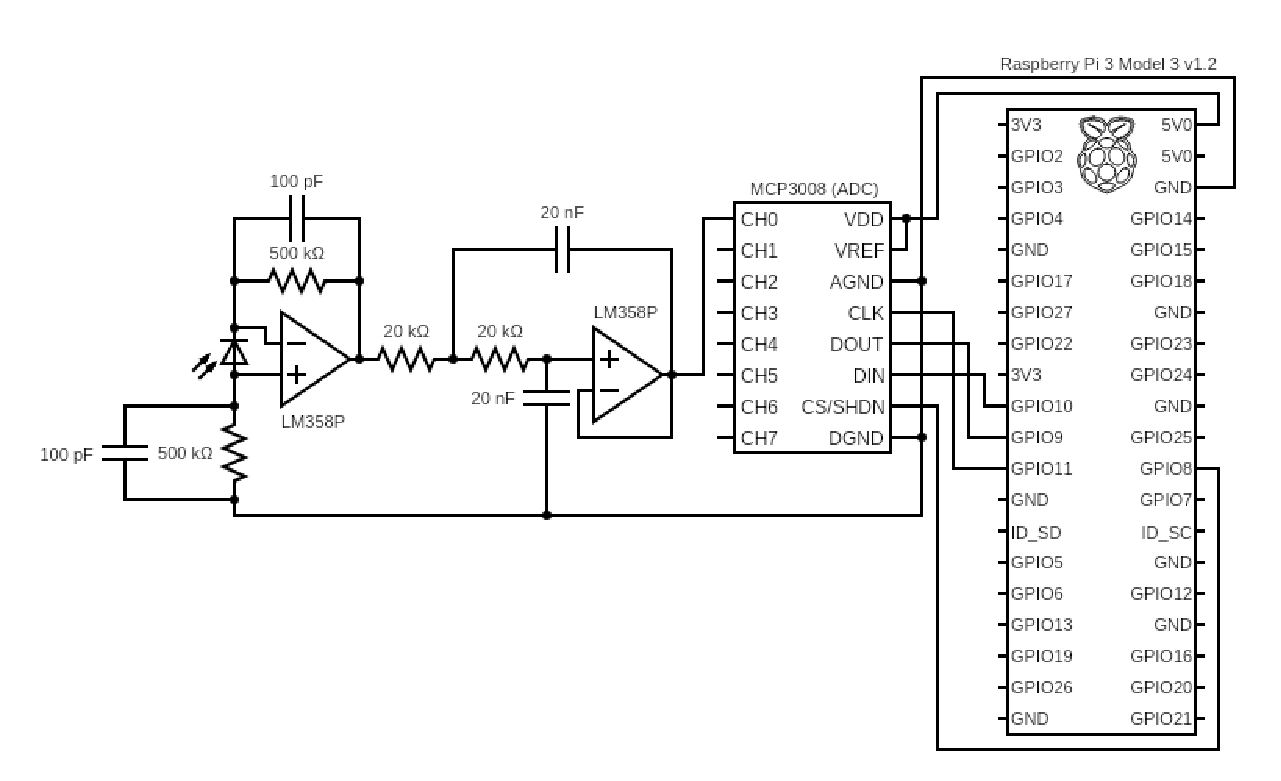
\includegraphics[width=\textwidth]{circuit_diagram.pdf}
	\caption{Circuit diagram for photo-diode reading. Photo-diode in reverse-bias over an op-amp, analog signal then passed through Sallen-Key anti-aliasing filter tuned to 16kHz, then into an analog-to-digital converter (ADC), that’s finally read by the special purpose input (SPI) pins of a Raspberry Pi}
	\label{fig:circuit_diagram}
\end{figure}



\begin{acknowledgments}
The authors are grateful to Robin Evans, Bill Moran, Jude Prezens, Alex Tolotchkoc, and Blake Molyneux for their technical advice and generous assistance throughout the project.
	
The authors are also grateful to Deeksha Beniwal, Sebastian Ng, and Craig Ingram for their advice and work in designing the interferometer. 

This research is supported by the Australian Research Council Centre of Excellence for Gravitational Wave Discovery (OzGrav) (project number CE170100004) and the Institute of Physics International Member Grant.

Travel during the project was supported by the Australian National University PhB Science  program.

\end{acknowledgments}


\bibliographystyle{myunsrt}
\bibliography{ifoDemoBib}

\end{document}
